\documentclass[11pt,a4paper]{article}

% --------------------------------------------------
% Packages
% --------------------------------------------------
\usepackage[utf8]{inputenc}
\usepackage[T1]{fontenc}
\usepackage[french]{babel}

\usepackage[a4paper,margin=2.5cm]{geometry}
\usepackage{setspace}
\usepackage{parskip}
\setlength{\parindent}{0pt}
\onehalfspacing

\usepackage{amsmath}
\usepackage{array}
\usepackage{booktabs}
\usepackage{tabularx}
\usepackage{multirow}

\usepackage{graphicx}
\usepackage{float}
\usepackage{caption}
\usepackage{subcaption}

\usepackage[hidelinks]{hyperref}
\usepackage{enumitem}
\usepackage{fancyhdr}
\usepackage{titlesec}
\usepackage{xcolor}

% --------------------------------------------------
% Chemin des images
% --------------------------------------------------
\graphicspath{{img/}}

% --------------------------------------------------
% Mise en page
% --------------------------------------------------
\pagestyle{fancy}
\fancyhf{}
\fancyhead[L]{TP1 -- Green IT}
\fancyhead[R]{Polytech Lyon}
\fancyfoot[C]{\thepage}

\newcolumntype{Y}{>{\raggedright\arraybackslash}X}

\titleformat{\section}{\large\bfseries}{\thesection}{1em}{}
\titleformat{\subsection}{\normalsize\bfseries}{\thesubsection}{1em}{}

% --------------------------------------------------
% Titre
% --------------------------------------------------
\title{
\textbf{TP1 -- Écoconception Web}\\
\large Analyse de l'impact environnemental d'un site web et proposition d'une version écoconçue
}

\author{
Nom Prénom 1 \\
Nom Prénom 2
}

\date{Mars 2026}

% --------------------------------------------------
\begin{document}

\maketitle
\thispagestyle{empty}

\vspace{0.8cm}

\begin{center}
\begin{tabular}{ll}
Formation : & Polytech Lyon -- 4A Informatique \\
Matière : & Green IT / Numérique responsable \\
Enseignant : & F. Perraud \\
Sujet : & Étude d'un site web et proposition d'une version écoconçue
\end{tabular}
\end{center}

\vfill

\begin{abstract}
Ce rapport présente l'étude environnementale de la page d'accueil du site Basic-Fit. L'analyse repose sur plusieurs outils de mesure d'impact écologique, notamment EcoIndex et WebsiteCarbon, ainsi que sur un audit technique mené à l'aide des outils de développement du navigateur. Les résultats mettent en évidence plusieurs mauvaises pratiques d'écoconception : poids élevé de la page, grand nombre de requêtes HTTP et structure DOM très complexe. Une refonte écoconçue de la page d'accueil est ensuite proposée et pourra être implémentée sous la forme d'une version HTML/CSS légère.
\end{abstract}

\newpage
\tableofcontents
\newpage

% --------------------------------------------------
\section{Introduction}

Le numérique occupe aujourd'hui une place centrale dans notre société. Les services web sont devenus indispensables dans de nombreux domaines comme l'éducation, l'administration, le commerce ou la communication. Cependant, cette généralisation du numérique s'accompagne d'un impact environnemental important.

Selon plusieurs études, le numérique représente aujourd'hui environ 4\,\% des émissions mondiales de gaz à effet de serre et près de 10\,\% de la consommation électrique mondiale. Le poids moyen des pages web a fortement augmenté au cours des dernières décennies, entraînant une sollicitation croissante des réseaux, des serveurs et des terminaux utilisateurs.

L'écoconception web consiste à réduire la quantité de ressources nécessaires au fonctionnement d'un service numérique tout en conservant une qualité de service acceptable pour l'utilisateur. Cette démarche repose notamment sur les principes de simplicité, frugalité et pertinence.

Dans le cadre de ce TP, l'objectif est d'analyser l'impact environnemental d'un site web existant, d'identifier ses principales mauvaises pratiques puis de proposer une version écoconçue de la page d'accueil.

% --------------------------------------------------
\section{Présentation du site étudié}

Le site choisi pour cette étude est le site institutionnel et commercial de Basic-Fit :

\begin{center}
\url{https://www.basic-fit.com}
\end{center}

Plus précisément, l'analyse porte sur la \textbf{page d'accueil} du site.

Ce site a pour objectif de présenter :
\begin{itemize}
\item l'offre commerciale de Basic-Fit
\item les abonnements proposés
\item les services disponibles
\item les clubs et équipements
\item différents contenus marketing destinés à convaincre l'utilisateur
\end{itemize}

Les principaux utilisateurs du site sont les visiteurs souhaitant découvrir l'offre, comparer les abonnements ou s'inscrire.

La page d'accueil constitue la principale porte d'entrée du site et concentre de nombreux contenus visuels, sections promotionnelles et éléments interactifs. C'est donc cette page qui a été retenue pour l'analyse.

% --------------------------------------------------
\section{Méthodologie}

L'étude a été réalisée en deux étapes principales :

\begin{itemize}
\item mesure de l'impact environnemental avec EcoIndex et WebsiteCarbon
\item audit technique via les outils de développement du navigateur
\end{itemize}

L'onglet \texttt{Network} de Chrome DevTools permet ensuite d'analyser plus finement :
\begin{itemize}
\item le nombre de requêtes HTTP
\item le nombre d'images
\item les scripts JavaScript chargés
\item les polices utilisées
\item la structure générale des ressources téléchargées
\end{itemize}

Dans cette première partie du travail, nous nous concentrons sur les résultats de mesure fournis par EcoIndex et WebsiteCarbon.

% --------------------------------------------------
\section{Analyse de l'impact environnemental}

\subsection{Résultats EcoIndex}

L'analyse de la page d'accueil de Basic-Fit avec EcoIndex donne les résultats suivants :

\begin{table}[H]
\centering
\caption{Résultats EcoIndex de la page d'accueil de Basic-Fit}
\begin{tabular}{lc}
\toprule
Indicateur & Valeur \\
\midrule
Score EcoIndex & 17 / 100 \\
Classe & F \\
Poids de page & 6.017 MB \\
Requêtes HTTP & 98 \\
Nombre d'éléments DOM & 3211 \\
\bottomrule
\end{tabular}
\end{table}

Ces résultats montrent que la page présente un impact environnemental important. Le score de 17/100 est particulièrement faible et classe la page dans la catégorie F.

Le poids de la page dépasse 6 MB, ce qui est très élevé pour une page d'accueil. Ce volume de données entraîne une consommation importante de bande passante et d'énergie.

Le nombre de requêtes HTTP est également élevé avec 98 requêtes, ce qui multiplie les échanges entre le navigateur et le serveur.

Enfin, la complexité du DOM est très importante avec plus de 3200 éléments, ce qui augmente fortement le coût de rendu côté navigateur.

\subsection{Résultats WebsiteCarbon}

L'analyse avec WebsiteCarbon attribue au site la note \textbf{B}. L'outil indique que la page est plus propre que \textbf{74\,\% des pages web}.

Ce résultat semble à première vue contradictoire avec le score EcoIndex de F. Cette différence s'explique par le fait que les deux outils utilisent des méthodologies différentes.

WebsiteCarbon se concentre principalement sur les émissions de CO\textsubscript{2} liées au transfert de données et à l'hébergement, tandis qu'EcoIndex prend aussi en compte la complexité du DOM et le nombre de requêtes HTTP. Ainsi, un site peut avoir un score relativement correct sur WebsiteCarbon tout en restant mauvais du point de vue de l'écoconception front-end.

\subsection{Empreinte environnementale estimée}

Selon EcoIndex, pour 1000 visites mensuelles, la page représenterait environ :

\begin{itemize}
\item 39.9 litres d'eau bleue consommés
\item 2.66 kgCO2e émis
\end{itemize}

Ces estimations permettent de mieux visualiser l'impact réel d'une page web lourde et complexe.

\subsection{Interprétation des résultats}

Les résultats montrent que la page d'accueil du site Basic-Fit présente plusieurs problèmes du point de vue de l'écoconception :

\begin{itemize}
\item un poids de page très élevé
\item une complexité DOM excessive
\item un nombre important de requêtes HTTP
\end{itemize}

Ces éléments indiquent que la page n'a pas été conçue dans une logique de sobriété numérique, mais plutôt dans une logique marketing privilégiant le visuel et l'expérience utilisateur.

La forte complexité du DOM, avec 3211 éléments, est particulièrement problématique. Elle impacte directement les performances du navigateur et la consommation de ressources côté client.

Le poids élevé de la page suggère également la présence de nombreuses images ou médias lourds, typiques des sites de communication et de promotion commerciale.

% --------------------------------------------------
\section{Captures des résultats}

\subsection{Résultat global EcoIndex}

\begin{figure}[H]
\centering
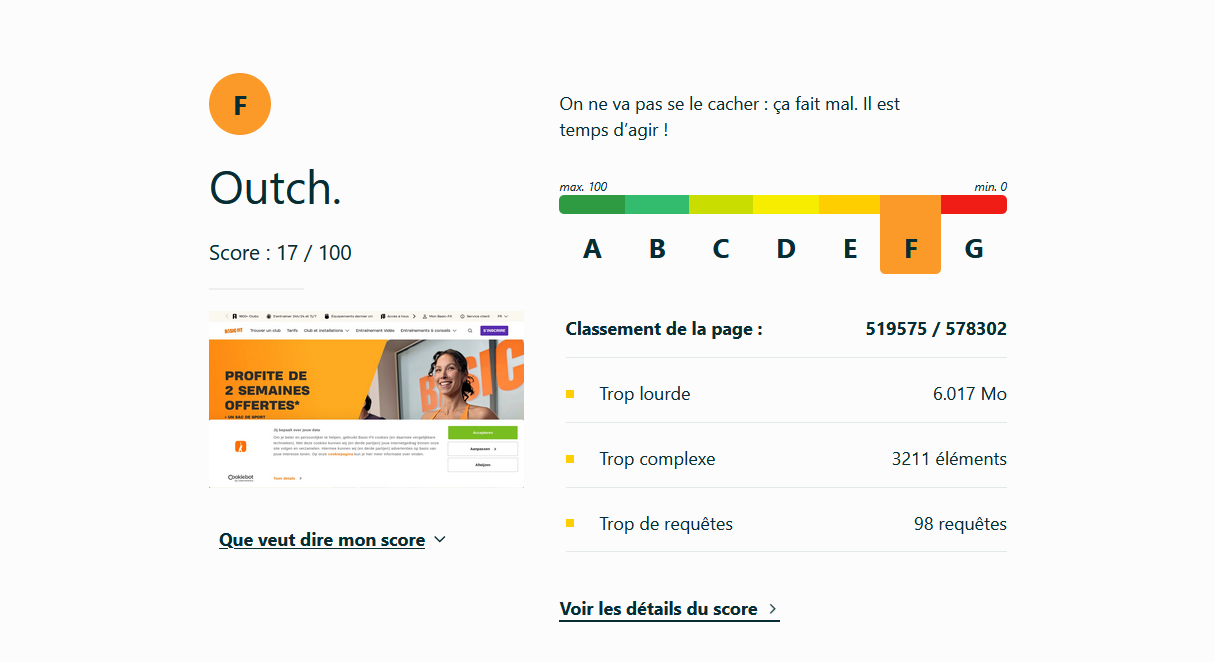
\includegraphics[width=0.85\textwidth]{ecoindex_global.png}
\caption{Résultat global EcoIndex de la page d'accueil de Basic-Fit}
\end{figure}

\subsection{Détails du score EcoIndex}

\begin{figure}[H]
\centering
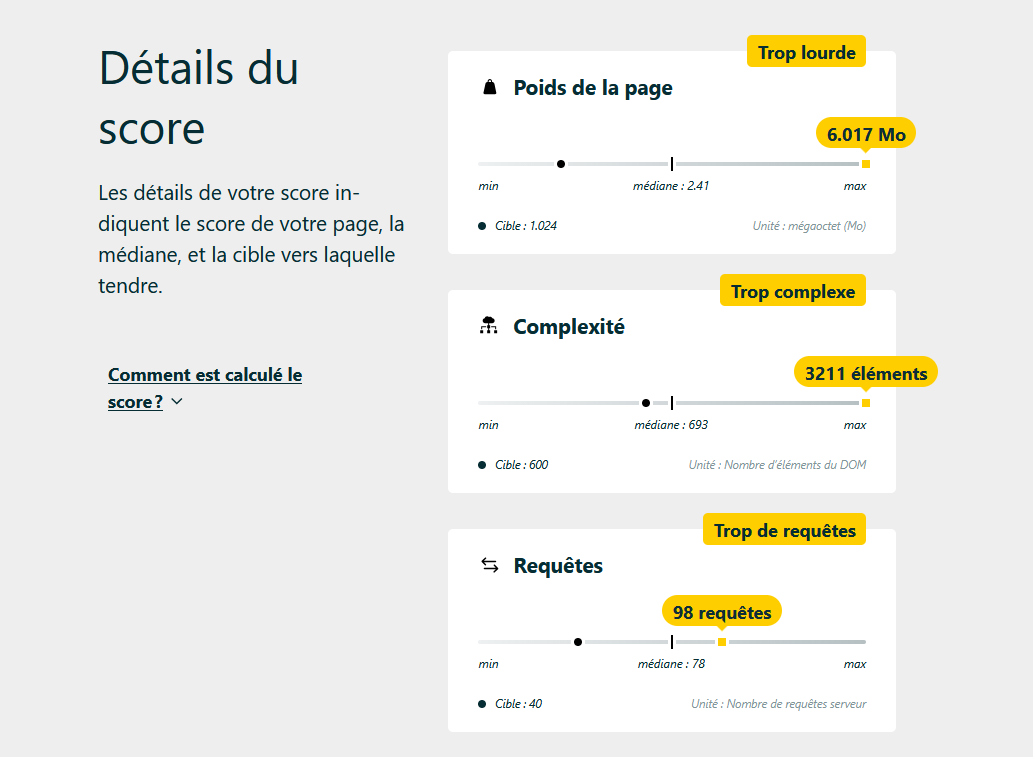
\includegraphics[width=0.85\textwidth]{ecoindex_details.png}
\caption{Détails du score EcoIndex : poids, complexité et nombre de requêtes}
\end{figure}

\subsection{Empreinte environnementale estimée}

\begin{figure}[H]
\centering
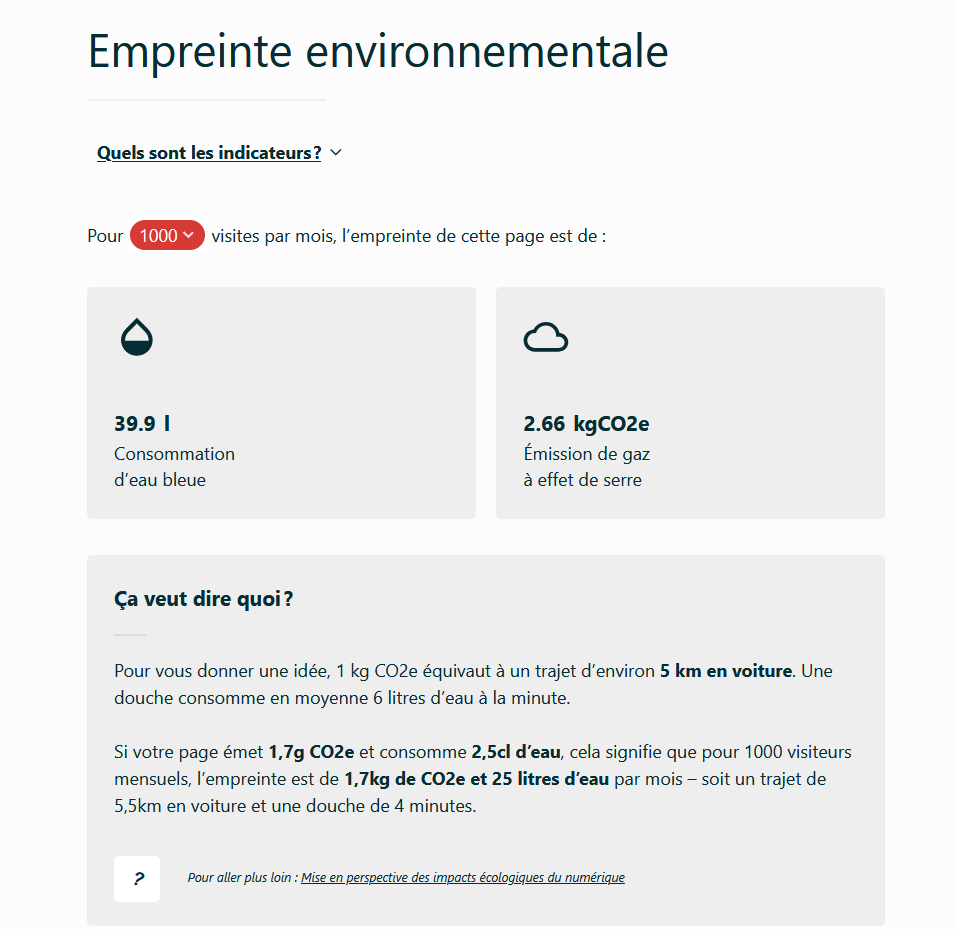
\includegraphics[width=0.85\textwidth]{ecoindex_empreinte.png}
\caption{Empreinte environnementale estimée selon EcoIndex}
\end{figure}

\subsection{Résultat WebsiteCarbon}

\begin{figure}[H]
\centering
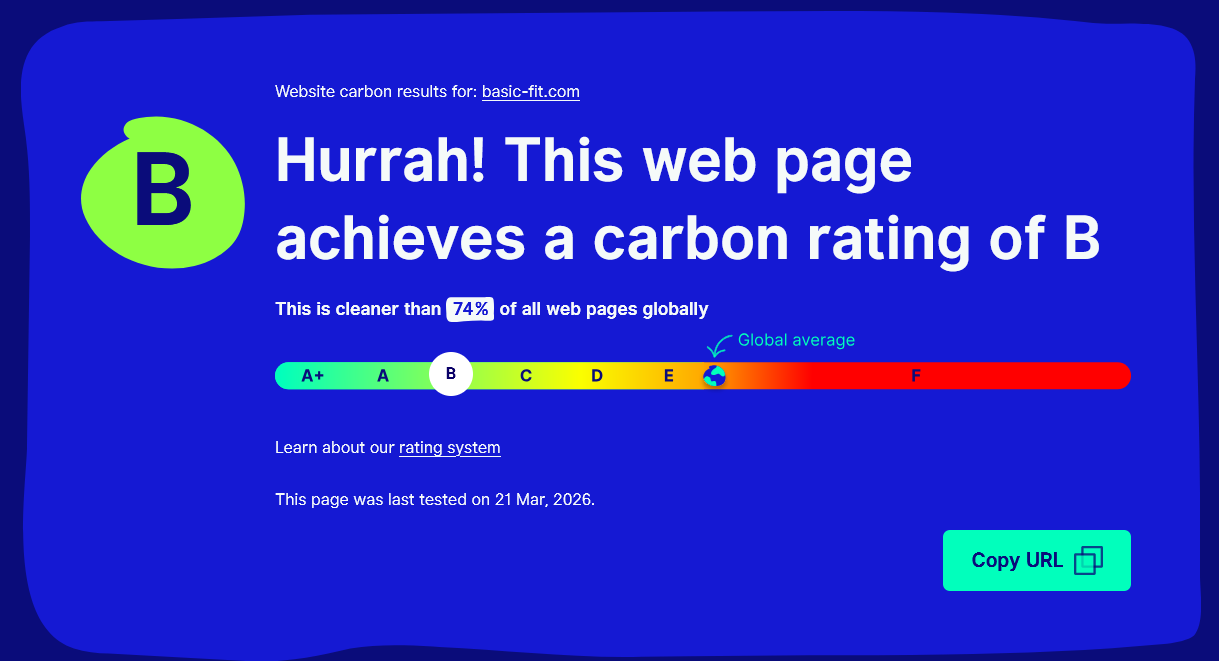
\includegraphics[width=0.85\textwidth]{websitecarbon.png}
\caption{Résultat WebsiteCarbon de la page d'accueil de Basic-Fit}
\end{figure}

% --------------------------------------------------
\section{Première synthèse}

À ce stade de l'étude, les résultats permettent déjà d'identifier plusieurs points faibles majeurs :

\begin{itemize}
\item la page est \textbf{très lourde} avec plus de 6 MB transférés
\item la page est \textbf{très complexe} avec plus de 3200 éléments DOM
\item la page nécessite \textbf{de nombreuses requêtes} pour être chargée
\end{itemize}

Ces constats montrent que la page d'accueil de Basic-Fit constitue un bon support d'étude pour un travail d'écoconception. La prochaine étape consistera à réaliser un audit technique plus détaillé à l'aide des outils de développement du navigateur afin d'identifier les causes précises de cette lourdeur.

% --------------------------------------------------
\section{Conclusion}

Cette première phase d'analyse met en évidence un impact environnemental important de la page d'accueil de Basic-Fit. Malgré une note WebsiteCarbon relativement correcte, le score EcoIndex est très faible et révèle une page lourde, complexe et coûteuse du point de vue du rendu navigateur.

L'étape suivante consistera à analyser plus finement les ressources réellement chargées par la page afin d'identifier les mauvaises pratiques techniques responsables de cette situation.

% --------------------------------------------------
\section{Bibliographie}

\begin{itemize}
\item ADEME -- \textit{La face cachée du numérique}
\item GreenIT.fr -- Référentiel d'écoconception web
\item EcoIndex -- \url{https://www.ecoindex.fr}
\item WebsiteCarbon -- \url{https://www.websitecarbon.com}
\item Support de cours Green IT / Numérique responsable
\item Sujet de TP -- Étude d'un site web
\end{itemize}

% --------------------------------------------------
\appendix

\section{Organisation conseillée du dossier}

\begin{verbatim}
rapport/
 ├ rapport_greenIT.tex
 └ img/
     ├ ecoindex_global.png
     ├ ecoindex_details.png
     ├ ecoindex_empreinte.png
     └ websitecarbon.png
\end{verbatim}

\section{Captures utilisées}

Les images suivantes doivent être placées dans le dossier \texttt{img/} :

\begin{itemize}
\item ecoindex_global.png
\item ecoindex_details.png
\item ecoindex_empreinte.png
\item websitecarbon.png
\end{itemize}

\end{document}